% Author: Marek Fiser <tikz at marekfiser.cz>
% MESIF protocol: http://en.wikipedia.org/wiki/MESIF_protocol
\documentclass[tikz, border=0pt]{standalone}
%%%<
\usepackage{verbatim}
%%%>
\usetikzlibrary{positioning}
\usetikzlibrary{shapes,snakes}
%% Define some nice colors
\definecolor{myBlue}{RGB}{85,173,228}
\definecolor{myGray1}{RGB}{208,206,206}
\definecolor{myGray2}{RGB}{175,171,171}
\definecolor{myGray3}{RGB}{127,127,127}
\begin{comment}
Made by: Johannes Borgqvist
Date: 2020-04-20
Description: 
We draw the reaction scheme for the activation scheme 
of cdc42
\end{comment}
\usetikzlibrary{arrows}
\begin{document}
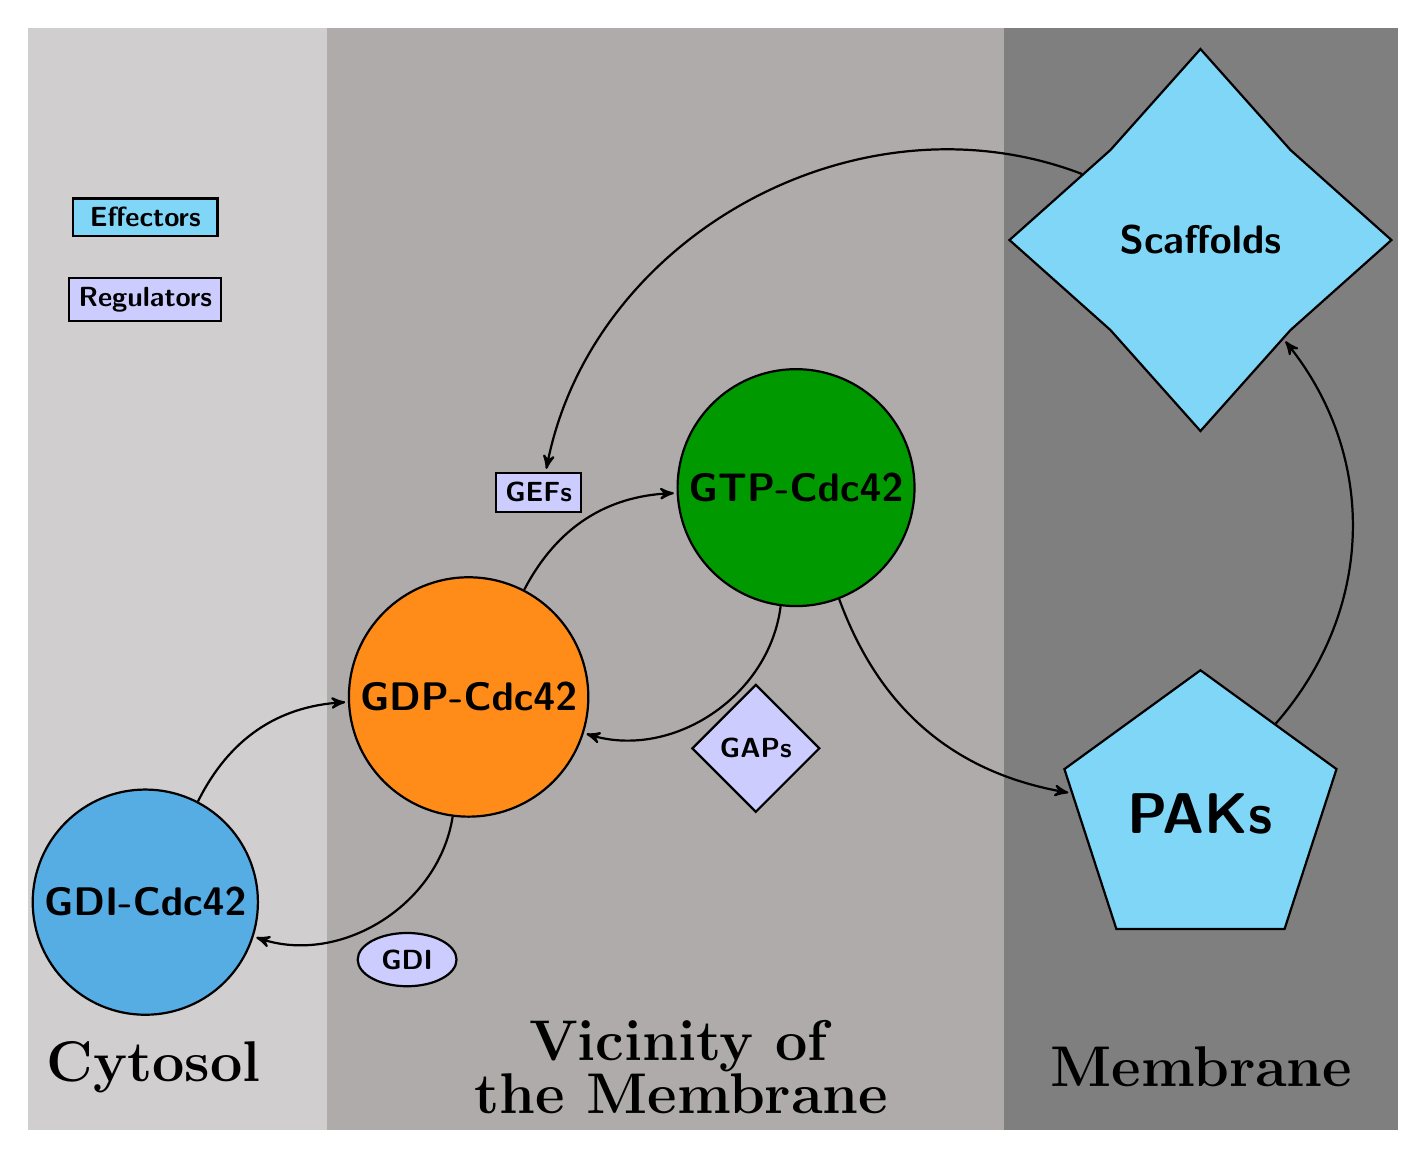
\begin{tikzpicture}[->,>=stealth',shorten >=1pt,auto,node distance=3cm,
  thick,main node/.style={circle,fill=green!60!black,draw,
  font=\sffamily\Large\bfseries,minimum size=2cm},second node/.style={circle,fill=orange!90,draw,
  font=\sffamily\Large\bfseries,minimum size=2cm},third node/.style={circle,fill=myBlue,draw,
  font=\sffamily\Large\bfseries,minimum size=2cm},small rect/.style={rectangle,fill=blue!20,draw,
  font=\sffamily\normalsize\bfseries,minimum size=0.5cm},small diamond/.style={diamond,fill=blue!20,draw,
  font=\sffamily\normalsize\bfseries,minimum size=0.5cm},small ellipse/.style={ellipse,fill=blue!20,draw,
  font=\sffamily\normalsize\bfseries,minimum size=0.5cm},PAK shape/.style={regular polygon,regular polygon sides=5,fill=cyan!50,draw,
  font=\sffamily\huge\bfseries,minimum size=2cm},Scaffold shape/.style={star,star points=4,fill=cyan!50,draw,
  font=\sffamily\Large\bfseries,minimum size=2cm},explanation 1/.style={rectangle,fill=cyan!50,draw,
  font=\sffamily\normalsize\bfseries,minimum size=0.1cm},explanation 2/.style={rectangle,fill=blue!20,draw,
  font=\sffamily\normalsize\bfseries,minimum size=0.1cm}]

  \begin{scope}
\path[fill=myGray3,opacity=1.0] (6.8,-5.5) -- (6.8,8.5) -- (11.8,8.5) -- (11.8,-5.5);
\path[fill=myGray2,opacity=1.0] (-1.8,-5.5) -- (-1.8,8.5) -- (6.8,8.5) -- (6.8,-5.5);
\path[fill=myGray1,opacity=1.0] (-5.6,-5.5) -- (-5.6,8.5) -- (-1.8,8.5) -- (-1.8,-5.5);
  \end{scope}
  
% The reaction scheme
  \node[second node] (I) {GDP-Cdc42};
  \node[main node] (A) [above right =0.5cm and 2cm of I] {GTP-Cdc42};
  \node[third node] (H) [below left =0.5cm and 2cm of I] {GDI-Cdc42};
  \node[small rect] (GEF) [above right =1.25cm and -0.75cm of I] {GEFs};
  \node[small diamond] (GAP) [above right =-2.15cm and 2.15cm of I] {GAPs};
  \node[small ellipse] (GDI) [above right =-2cm and 1.85cm of H] {GDI};
  \node[PAK shape] (PAK) [below right =2cm and 3cm of A] {PAKs};
  \node[Scaffold shape] (Scaffold) [above =3cm of PAK] {Scaffolds};
\node [explanation 1] (Effectors)[above =7cm of H] {$\;$Effectors$\;$};
\node [explanation 2] (Regulators)[below =0.5cm of Effectors] {Regulators};
%\node at (2.4,-4.3) {\huge\textbf{Vicinity of}};
%\node at (2.7,-5) (Cytosol){\huge\textbf{the Membrane}};
\node[align=center] at (2.7,-4.7) (Cytosol){\huge\textbf{Vicinity of}\\\huge\textbf{the Membrane}};
\node (Membrane) [right=1.8cm of Cytosol]{\huge\textbf{Membrane}};
\node at (-4.0,-4.7) (Cytosol){\huge\textbf{Cytosol}};
% The Arrows between the nodes
 \path[every node/.style={font=\sffamily\small,inner sep=0pt}]
 (A) edge [bend left=50] node {\color{myGray2}} (I)% Activation
 (I) edge [bend left] node {} (A)
 (I) edge [bend left=50] node {} (H)
 (H) edge [bend left] node {} (I)
 (A) edge [bend right=30] node {} (PAK)
 (PAK) edge [bend right=40] node {} (Scaffold)
 (Scaffold) edge [bend right=50] node {} (GEF);





\end{tikzpicture}
\end{document}
